\documentclass{article}
\usepackage{graphicx}
\usepackage{listings}
\usepackage{ctex}
\usepackage{graphicx}
\usepackage[a4paper, body={18cm,22cm}]{geometry}
\usepackage{amsmath,amssymb,amstext,wasysym,enumerate,graphicx}
\usepackage{float,abstract,booktabs,indentfirst,amsmath}
\usepackage{array}
\usepackage{booktabs} %调整表格线与上下内容的间隔
\usepackage{multirow}
\usepackage{diagbox}
\usepackage{indentfirst}
\usepackage{bm}
\usepackage{fancyhdr}




\pagestyle{fancy}

\lhead{\bfseries \normalsize 学号:1952033\quad 姓名:侯雅玥 \quad 组员:廖宏 \\实验名称:集成移位寄存器应用实验\quad 课程名称:电子技术实验\quad 专业:微电子科学与工程 } 
\rhead{}

\begin{document}
	\section{\zihao{4} 实验名称:集成移位寄存器应用实验}
    \section{\zihao{4} 实验目的}
    \zihao {5} (1) 了解集成移位寄存器的控制功能。\par 
               (2)掌握集成移位寄存器的应用。\par
   	\section{\zihao{4} 实验原理}
      
       移位寄存器的功能是当时钟控制脉冲有效时,寄存器中存储的数码同时顺序向高位(左移)或向低位(右移)移动一位。所以,移位寄存器的各触发器状态必须同时变化,为同步时序电路。\par
       因为数据可以按序逐位从最低位或最高位串行输入移位寄存器,也可以通过置数端并行输入移位寄存器。所以移位寄存器的数据输入、输出方式有并行输入/并行输出、并行输入/串行输出、串行输入/并行输出、串行输入/串行输出。
       移位寄存器主要应用于实现数据传输方式的转换(串行到并行或并行到串行)、脉冲分配、序列信号产生以及时序电路的周期性循环控制(计数器)等。
       4 位移位寄存器 74LS194 的逻辑功能如表1所示。在方式信号 $S_i$和$ S_A$控制下,74LS194可以实现右移(串行数据从 $S_D$输入)、左移(串行数据从 $ S_A$输入)、置数(并行数据从d,c,b,a 输入)及保持(输出不变)功能。
       \begin{figure*}[h]
        %\small
        \centering
        \includegraphics[width=3.5in]{H:/电子技术试验/4-22/4-22-3.jpg}
        \caption{4位移位寄存器74LS194功能表} \label{fig:aa}
        \end{figure*}
   \newpage    
\section{\zihao{4}实验电路}

       图1为简易乒乓球游戏机电路。输入 R,L为球拍击球信号,高电平有效,输出 QD~QA,接4个发光二极管指示乒乓球的运动轨迹。游戏规则∶R或L输入一个正脉冲发球,发光二极管指示球向对方移动,到达对方顶端位置时,对方必须及时接球,使球返回,否则就会失球。输入的移位脉冲频率越高,球的移动轨迹越快,接球难度越大。
       \begin{figure}[h]
        %\small
        \centering
        \includegraphics[width=3.5in]{H:/电子技术试验/4-22/4-22-1.png}
        \caption{乒乓球电路} \label{fig:aa}
        \end{figure}
       
       图2为移存型计数器
       \begin{figure}[h]
        %\small
        \centering
        \includegraphics[width=3.5in]{H:/电子技术试验/4-22/4-22-2.png}
        \caption{移存型计数器电路} \label{fig:aa}
        \end{figure}
       图3(a)、图3(b)分别为左移环形计数器和右移环形计数器
       \begin{figure}[h]
        \begin{minipage}[t]{0.5\linewidth} % 如果一行放2个图,用0.5,如果3个图,用0.33  
          \centering   
          \includegraphics[width=3.5in]{H:/电子技术试验/4-22/4-22-3.png}   
          \caption{$CLK/Q0$}   
          \label{fig:side:a}   
        \end{minipage}%   
        \begin{minipage}[t]{0.5\linewidth}   
          \centering   
          \includegraphics[width=3.5in]{H:/电子技术试验/4-22/4-22-4.png}   
          \caption{$CLK/Q1$}   
          \label{fig:side:b}   
        \end{minipage}   
      \end{figure}
      \begin{figure}[h]
        %\small
        \centering
        \includegraphics[width=3.5in]{H:/电子技术试验/4-22/4-22-5.png}
        \caption{74LS194引脚图} \label{fig:aa}
        \end{figure}

\section{\zihao{4} 实验内容及步骤}
1.按表1验证74LS194的功能。\par
2.按图1接线,观察乒乓球游戏电路的效果。\par
3.移存型计数器:连接图2电路。电路复位后输入1Hz时钟,观察电路输出状态是否与理论分析相同。时钟改为10kHz,用示波器记录Q3—Q0的输出序列信号的波形。\par
4.74LS194构成的4位环形计数器:连接电路,预置初值“0001”,时钟为10kHz,用示波器观察和记录CP,Q3—Q0的波形图。\par



\section{\zihao{4} 实验设备和器材}
(1)直流稳压电源              \qquad \quad \qquad \qquad \qquad \qquad           1台\par
(2)数字逻辑实验箱            \qquad  \qquad \qquad \qquad\qquad                1台\par
(3)74LS00、74LS161、74LS194              \quad                                    若干片\par
(4)示波器                   \qquad  \qquad \qquad \qquad\qquad  \qquad  \qquad    1台\par
(5)导线   
\section{\zihao{4} 数据及误差处理}
(1)乒乓球电路\par
如图进行仿真,仿真结果符合预期


(2)移存型计数器
Q3—Q0的输出状态:  \par
1Hz:经实验观察,符合预期\par
1kHz,cp,Q1~Q3如下:
\begin{figure}[h]
    \begin{minipage}[t]{0.5\linewidth} % 如果一行放2个图,用0.5,如果3个图,用0.33  
      \centering   
      \includegraphics[width=3in]{H:/电子技术试验/4-22/SCR11.png}   
      \caption{CP/Q0}   
      \label{fig:side:a}   
    \end{minipage}%   
    \begin{minipage}[t]{0.5\linewidth}   
      \centering   
      \includegraphics[width=3in]{H:/电子技术试验/4-22/SCR12.png}   
      \caption{Q0/Q1}   
      \label{fig:side:b}   
    \end{minipage}   
\end{figure}
    \begin{figure}[h]
        \begin{minipage}[t]{0.5\linewidth} % 如果一行放2个图,用0.5,如果3个图,用0.33  
          \centering   
          \includegraphics[width=3in]{H:/电子技术试验/4-22/SCR14.png}   
          \caption{Q1/Q2}   
          \label{fig:side:a}   
        \end{minipage}%   
        \begin{minipage}[t]{0.5\linewidth}   
          \centering   
          \includegraphics[width=3in]{H:/电子技术试验/4-22/SCR15.png}   
          \caption{Q2/Q3}   
          \label{fig:side:b}   
        \end{minipage}   .
    \end{figure}
    \newpage
    得到时序图:
    \begin{figure}[h]
        %\small
        \centering
        \includegraphics[width=3.5in]{H:/电子技术试验/4-22/4-22-8.png}
        \caption{移存型计数器时序图} \label{fig:aa}
        \end{figure}

左移环形计数器:
按下图仿真:
\begin{figure}[h]
    %\small
    \centering
    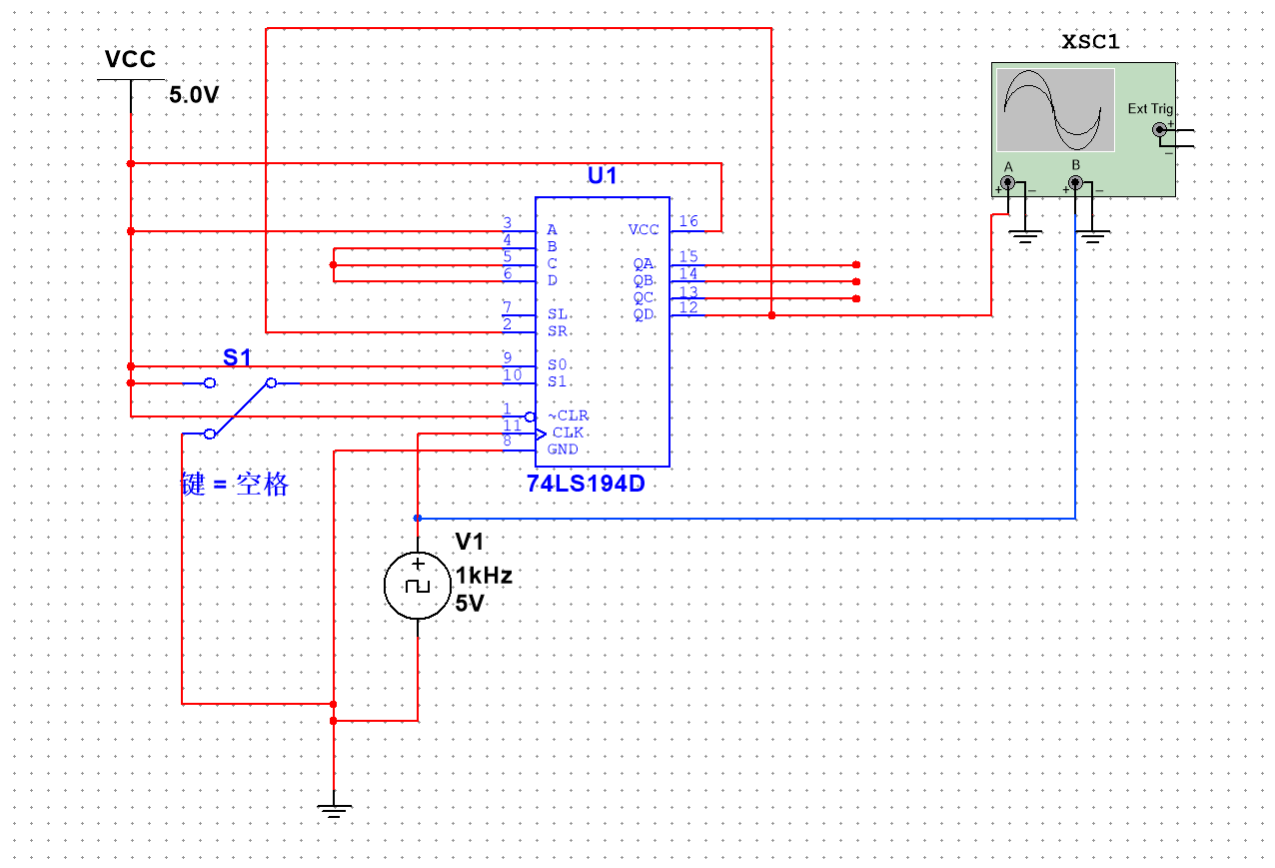
\includegraphics[width=3in]{H:/电子技术试验/4-22/4-22-6.png}
    \caption{移存型计数器时序图} \label{fig:aa}
    \end{figure}
\newpage
1Hz:经实验观察,符合预期\par
1kHz,cp,Q1~Q3如下:
\begin{figure}[h]
    \begin{minipage}[t]{0.5\linewidth} % 如果一行放2个图,用0.5,如果3个图,用0.33  
      \centering   
      \includegraphics[width=3.2in]{H:/电子技术试验/4-22/1-1.png}   
      \caption{CP/Q0}   
      \label{fig:side:a}   
    \end{minipage}%   
    \begin{minipage}[t]{0.5\linewidth}   
      \centering   
      \includegraphics[width=3.5in]{H:/电子技术试验/4-22/1-2.png}   
      \caption{Q0/Q1}   
      \label{fig:side:b}   
    \end{minipage}   
\end{figure}
    \begin{figure}[h]
        \begin{minipage}[t]{0.5\linewidth} % 如果一行放2个图,用0.5,如果3个图,用0.33  
          \centering   
          \includegraphics[width=3.5in]{H:/电子技术试验/4-22/1-3.png}   
          \caption{Q1/Q2}   
          \label{fig:side:a}   
        \end{minipage}%   
        \begin{minipage}[t]{0.5\linewidth}   
          \centering   
          \includegraphics[width=3.5in]{H:/电子技术试验/4-22/1-4.png}   
          \caption{Q2/Q3}   
          \label{fig:side:b}   
        \end{minipage}   .
    \end{figure}
    \newpage
得到时序图:
\begin{figure}[h]
    %\small
    \centering
    \includegraphics[width=3.5in]{H:/电子技术试验/4-22/4-22-11.png}
    \caption{移存型计数器时序图} \label{fig:aa}
    \end{figure}

右移环形计数器:
按下图仿真:
\begin{figure}[h]
    %\small
    \centering
    \includegraphics[width=3.5in]{H:/电子技术试验/4-22/4-22-7.png}
    \caption{移存型计数器时序图} \label{fig:aa}
    \end{figure}


1Hz:经实验观察,符合预期\par
\newpage
1kHz,cp,Q1~Q3如下:
\begin{figure}[h]
    \begin{minipage}[t]{0.5\linewidth} % 如果一行放2个图,用0.5,如果3个图,用0.33  
      \centering   
      \includegraphics[width=2.8in]{H:/电子技术试验/4-22/2-1.png}   
      \caption{CP/Q0}   
      \label{fig:side:a}   
    \end{minipage}%   
    \begin{minipage}[t]{0.5\linewidth}   
      \centering   
      \includegraphics[width=2.8in]{H:/电子技术试验/4-22/2-2.png}   
      \caption{Q0/Q1}   
      \label{fig:side:b}   
    \end{minipage}   
\end{figure}
    \begin{figure}[h]
        \begin{minipage}[t]{0.5\linewidth} % 如果一行放2个图,用0.5,如果3个图,用0.33  
          \centering   
          \includegraphics[width=2.8in]{H:/电子技术试验/4-22/2-3.png}   
          \caption{Q1/Q2}   
          \label{fig:side:a}   
        \end{minipage}%   
        \begin{minipage}[t]{0.5\linewidth}   
          \centering   
          \includegraphics[width=2.8in]{H:/电子技术试验/4-22/2-4.png}   
          \caption{Q2/Q3}   
          \label{fig:side:b}   
        \end{minipage}   .
    \end{figure}
得到时序图:
\begin{figure}[h]
    %\small
    \centering
    \includegraphics[width=2.8in]{H:/电子技术试验/4-22/4-22-9.png}
    \caption{移存型计数器时序图} \label{fig:aa}
    \end{figure}



\newpage
\section{结论}

74LS194的功能符合预期\par
\begin{figure}[h]
    %\small
    \centering
    \includegraphics[width=7in]{H:/电子技术试验/4-22/3-1.png}
    \caption{74LS194功能表} \label{fig:aa}
    \end{figure}
    移存型计数器时序图符合预期\par
\begin{figure}[h]
    %\small
    \centering
    \includegraphics[width=7in]{H:/电子技术试验/4-22/4-22-8.png}
    \caption{移存型计数器时序图} \label{fig:aa}
    \end{figure}
    \newpage
    左移寄存器的时序图:
    \begin{figure}[h]
        %\small
        \centering
        \includegraphics[width=7in]{H:/电子技术试验/4-22/4-22-11.png}
        \caption{左移寄存器的时序图} \label{fig:aa}
        \end{figure}
    右移寄存器的时序图:
    \begin{figure}[h]
        %\small
        \centering
        \includegraphics[width=7in]{H:/电子技术试验/4-22/4-22-9.png}
        \caption{右移寄存器的时序图} \label{fig:aa}
        \end{figure}

\end{document}